\section{Расчет УЭЦН}
Пользовательские функции связанные с расчетов установок электических центробежных насосов приведены в модуле «u7\_Excel\_functions\_ESP».  Названия функций начинаются с префикса ESP. 

УЭЦН состоит из следующих основных конструктивных элементов:
\begin{itemize}
	\item ЦН - центробежный насос. Модуль обеспечивающий перекачку жидкости за счет преобразования механической энергии вращения вала в гидравлическую мощность. 
	\item ПЭД - погружной электрический двигатель. Модуль обеспечивающий преобразование электрической энергии, поступающей по кабелю к погружному электрическому двигателю в механическую энергию вращения вала.
	\item ГС - газосепаратор или приемный модуль. Модуль обеспечивающий забор пластовой жидкости из скважины и подачу ее в насос. При этом центробежный газосепаратор способе отделить часть свободного газа в потоке и направить его в межтрубное пространство скважины. Работает за счет механической энергии вращения вала.
	\item вал - узел передающий энергию от погружного электрического двигателя (ПЭД) к остальным узлам установки, в том числе к центробежному насосу.
	\item кабель - узел передающий электрическую энергию с поверхности к погружному электрическому двигателю
	\item трансформатор - узел обеспечивающий необходимое напряжение на кабеле на поверхности. Как правило на вход трансформатора подается напряжение 380 В а на выходе оно поднимается до нескольких тысяч вольт. 
	\item СУ - станция управления ЭЦН. Узел управляющий работой системы УЭЦН. Может запускать останавливать скважины, обеспечивает защиту установки ЭЦН при нежелательных режимах работы
	\item ЧРП - частотно регулируемый привод. Обычно комплектуется со станцией управления УЭЦН. Обеспечивает изменение частоты колебаний напряжения и тока, а соответственно и частоты вращения вала ЭЦН. Может отсутствовать в компоновке УЭЦН. 
\end{itemize}

В промысловых сводках и отчетах часто ЭЦН обозначаются с использованием значений габарита насоса, номинальной подачи и номинального напора. ЭЦН5А 50 - 2000, означает что, это насос 5А габарита, с номинальной подачей 50 м3/сут и напором 2000 м. 

\begin{figure}[h!]
	\center{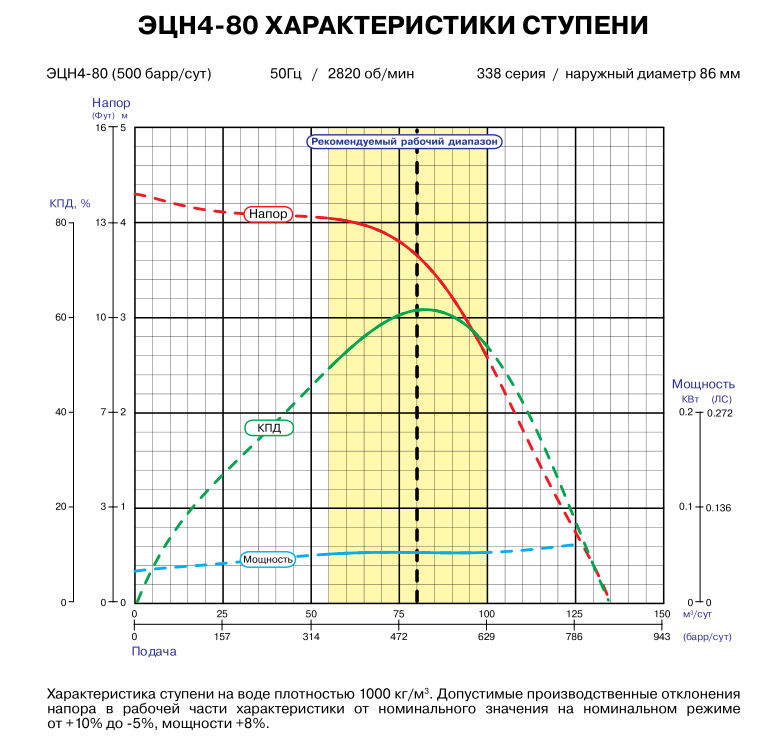
\includegraphics[width=0.8\linewidth]{novomet_ESP_80}}
	\caption{Пример каталожных характеристик ЭЦН}
	\label{ris:novomet_ESP_80}
\end{figure}

УЭЦН как и другие центробежные машины обладает относительно узким диапазоном подач при которых достигается достаточно высокий КПД его работы (от 30 до 60\%). В связи с этим для различных подач выпускаются различные типы УЭЦН. Всего в промышленности используются сотни различных типов ЭЦН различных производителей. Характеристики различных насосов предоставляются производителями в каталогах оборудования и обычно встраиваются в расчетным программы в виде баз данных характеристик оборудования. В надстройке \unf содержится база данных характеристик ЭЦН, которая может быть использована при проведении расчетов пользовательскими функциями. База сокращенная, содержит ряд насосов только одного производителя. Как правило этого достаточно для проведения базовых расчетов, так как характеристики насосов одного типоразмера разных производителей схожи между собой. 

Для выбора определенного насоса из базы необходимо использовать его идентификатор в базе - \mintinline{vb.net}{pump_id}

Задача расчета УЭЦН обычно сводится к следующим:
\begin{itemize}
	\item Прямая задача - по заданным значениям дебита жидкости скважины,  давлению на приеме, напряжению питания УЭЦН на поверхности найти давление на выкиде насоса, потребляемую электрическую мощность, потребляемый ток установки, КПД всей системы и отдельных узлов системы
	\item Обратная задача - по данным контроля параметров работы УЭЦН на поверхности - потребляемому току, напряжению питания частоте подаваемого напряжения, данным по конструкции УЭЦН и скважины найти дебит жидкости и обводнённость по скважине, давление на приеме и забойное давление.
	\item Задача узлового анализа - по данным конструкции скважины, параметров работы погружного оборудования оценить дебит по жидкости скважины при заданным параметрах работы УЭЦН или при из изменении. К этому типу задач относится задача подбора погружного оборудования для достижения заданных условий эксплуатации 
	
\end{itemize}

Для расчёта УЭЦН требуется рассчитать гидравлические параметры работы ЦН и электромеханические параметры ПЭД.

\subsection{ESP\_head\_m – расчёт номинального напора ЭЦН}
Функция позволяет получить паспортные характеристики ЭЦН - напор при определенной подаче. 

\putlisting{listings/ESP_head_m.lst}

Расчет выполняется на основе паспортных характеристик ЦН. 

\subsection{ESP\_eff\_fr – расчёт номинального КПД ЭЦН}
Функция позволяет получить паспортные характеристики ЭЦН - КПД  при определенной подаче. 

\putlisting{listings/ESP_eff_fr.lst}

Расчет выполняется на основе паспортных характеристик ЦН. 

\subsection{ESP\_power\_W – расчёт номинальной мощности потребляемой ЭЦН}
Функция позволяет получить паспортные характеристики ЭЦН - мощность потребляемая с вала при определенной подаче. 

\putlisting{listings/ESP_power_W.lst}

Расчет выполняется на основе паспортных характеристик ЦН. 

\subsection{ESP\_id\_by\_rate – выбор типового насоса по номинальному дебиту}
Функция возвращает идентификатор типового насоса по заданному номинальному дебиту. 
Может быть использована для выбора насоса на основе его наименования типа ЭЦН 50 - 2000.
\putlisting{listings/ESP_id_by_rate.lst}

\subsection{ESP\_dp\_atm – расчет перепада давления развиваемого ЭЦН}
Функция рассчитывает перепад давления развиваемый ЦН при заданных параметрах флюида и термобарических условиях.
\putlisting{listings/ESP_dp_atm.lst}

\subsection{ESP\_system\_calc – расчет параметров работы УЭЦН}
Функция рассчитывает полный набор параметров работы УЭЦН при заданных параметрах флюида и термобарических условиях. В отличии от функции  \mintinline{vb.net}{ESP\_dp\_atm} учиывает проскальзывание при расчете частоты вращения вала и рассчитываются электические параметры работы ЭЦН
\putlisting{listings/ESP_system_calc.lst}


\subsection{Электромеханический расчёт погружного электрического двигателя ПЭД}
Рассматривается асинхронный электрический двигатель. 

Погружные асинхронные электрические двигатели для добычи нефти выполяются трехфазными. 

Впервые конструкция трёхфазного асинхронного двигателя была разработана, создана и опробована русским инженером М. О. Доливо-Добровольским в 1889-91 годах. Демонстрация первых двигателей состоялась на Международной электротехнической выставке во Франкфурте на Майне в сентябре 1891 года. На выставке было представлено три трёхфазных двигателя разной мощности. Самый мощный из них имел мощность 1.5 кВт и использовался для приведения во вращение генератора постоянного тока. Конструкция асинхронного двигателя, предложенная Доливо-Добровольским, оказалась очень удачной и является основным видом конструкции этих двигателей до настоящего времени.

За прошедшие годы асинхронные двигатели нашли очень широкое применение в различных отраслях промышленности и сельского хозяйства. Их используют в электроприводе металлорежущих станков, подъёмно-транспортных машин, транспортёров, насосов, вентиляторов. Маломощные двигатели используются в устройствах автоматики.

Широкое применение асинхронных двигателей объясняется их достоинствами по сравнению с другими двигателями: высокая надёжность, возможность работы непосредственно от сети переменного тока, простота обслуживания.

Для расчёта электромеханических параметров погружных электрических двигателей полезно понимать теоретические основы их работы. Теория работы погружных асинхронных двигателей не отличаем от теории применимой к двигателям применяемым на поверхности. Далее кратко изложены основные положения теории. 

Трехфазная цепь является частным случаем многофазных систем электрических цепей, представляющих собой совокупность электрических цепей, в которых действуют синусоидальные ЭДС одинаковой частоты, отличающиеся по фазе одна от другой и создаваемые общим источником энергии.
Переменный ток протекающий по трехфазной цели характеризуется следующими параметрами:

\begin{itemize}
	\item Фазное напряжение $U_A, U_B, U_C $ - напряжение между линейным проводом и нейтралью
	\item Линейное напряжение $U_{AB}, U_{BC}, U_{CA} $ - напряжение между одноименными выводами разных фаз
	\item Фазный ток $I_{phase}$ – ток в фазах двигателя.
	\item Линейный ток $I_{line}$ – ток в линейных проводах.
	\item $ \cos \varphi $ - коэффициент мощности, где $ \varphi$ величина сдвига по фазе между напряжением и током 
\end{itemize}

Подключение двигателя к цепи трехфазного тока может быть выполнено по схеме "звезда" или "треугольник".

Тут нужен рисунок  

Для схемы звезда фазное напряжение меньше линейного в $\sqrt{3}$ раз.

$$ U_{AB} = \sqrt{3} U_{A} $$
$$ I_{phase} = I_{line} $$

Для схемы треугольник 

$$ U_{AB} =  U_{A} $$
$$ I_{line} =\sqrt{3} I_{phase} $$


В погружных двигателях обычно применяет схема подключения звезда. Эта схема обеспечивает более низкое напряжение в линии, что способствует повышению КПД передачи энергии по длинному кабелю. Еще есть причины?
При схеме подключения звезда токи в линии и в фазной обмотке статора двигателя совпадают, поэтому значение тока обозначают $I$ не указывая индекс в явном виде. Поскольку линейное напряжения проще измерить и легче контролировать параметры трехфазного двигателя обычно заданию линейный. в частности номинальное напряжение питания двигателя это линейное напряжение (напряжение между фазами). Далее линейное напряжение будет обозначать без индекса как $U$

Активная электрическая мощность в трехфазной цепи задается выражением 
$$ P= \sqrt{3}U I \cos \varphi$$

Реактивная мощность 
$$ Q= \sqrt{3}U I \sin \varphi$$

Соответственно полная мощность 
$$ S= \sqrt{3}U I $$

\subsubsection{ Устройство трёхфазной асинхронной машины}
Неподвижная часть машины называется статор, подвижная – ротор. Обмотка статора состоит из трёх отдельных частей, называемых фазами.

При подаче переменного напряжения и тока на обмотки статора внутри статора формируется вращающееся магнитное поле. Частота вращения магнитного поля совпадает с частотой питающего напряжения. 

Магнитный поток $\Phi $ и напряжение подаваемое на статор связаны приближенным соотношением 
$$ U_1 \approx E_1 = 4.44 w_1 k_1 f \Phi $$
где 

 $\Phi$ -  магнитный поток;
 
 $U_1$ -	напряжение в одной фазе статора;
 
 $f$   - частота сети;
 
 $E_1$	- ЭЦН в фазе статора;
 
 $w_1$ - число витков одной фазы обмотки статора;
 
 $k_1$  - обмоточный коэффициент.
   
Из этого выражения следует, что магнитный поток $\Phi $ в асинхронной машине не зависит от её режима работы, а при заданной частоте сети $f$ зависит только от действующего значения приложенного напряжения $U_1$


Для ЭДС ротора можно записать выражение 


$$  E_2 = 4.44 w_2 k_2 f S \Phi $$

где 


$S$ - величина скольжения (проскальзывания);

$E_2$	- ЭЦН в фазе ротора;

$w_2$ - число витков одной фазы обмотки ротора;

$k_2$ - обмоточный коэффициент ротора.

ЭДС, наводимая в обмотке ротора, изменяется пропорционально скольжению и в режиме двигателя имеет наибольшее значение в момент пуска в ход.
Для тока ротора в общем случае можно получить такое соотношение

$$  I_2 = \frac{E_2 S}{\sqrt{R_2^2+(S X_2^2)}} $$

где 

$R_2$ -  активное сопротивление обмотки ротора, связанное с потерями на нагрев обмотки;  

$X_2 = 2 \pi f L_2$ - индуктивное сопротивление обмотки неподвижного ротора, связанное с потоком рассеяния;

Отсюда следует, что ток ротора зависит от скольжения и возрастает при его увеличении, но медленнее, чем ЭДС.

Для асинхронного двигателя можно получить следующее выражение для механического момента 

$$ M = \frac{1}{4.44 w_2 k_2 k_T^2 f} \frac{U_1^2 R_2 S}{R_2^2 + (S X_2^2)^2}$$

где 

$k_T = \frac{E_1}{E_2} = \frac{w_1 k_1}{w_2 k_2}$ - коэффициент трансформации асинхронной машины

Из полученного выражения для электромагнитного момента следует, что он сильно зависит от подведённого напряжения ($M \sim U_1^2$). При снижении, например, напряжения на 10\%, электромагнитный момент снизится на 19\% $M \sim (0,9U_1)^2=0.81 U_1^2)$. Это является одним из недостатков асинхронных двигателей. 

Электромеханическая модель погружного АПЭД реализована в расчетных функциях \unf как модель двигателя с номером 0  \mintinline{vb.net}{motorID = 0}

Функции для расчета характеристик ПЭД начинаются с префикса \mintinline{vb.net}{motor_}. Описание функций можно найти в приложении "Автоматически сгенерированное описание".

\subsubsection{Каталожные характеристики АПЭД}

\begin{figure}[h!]
	\center{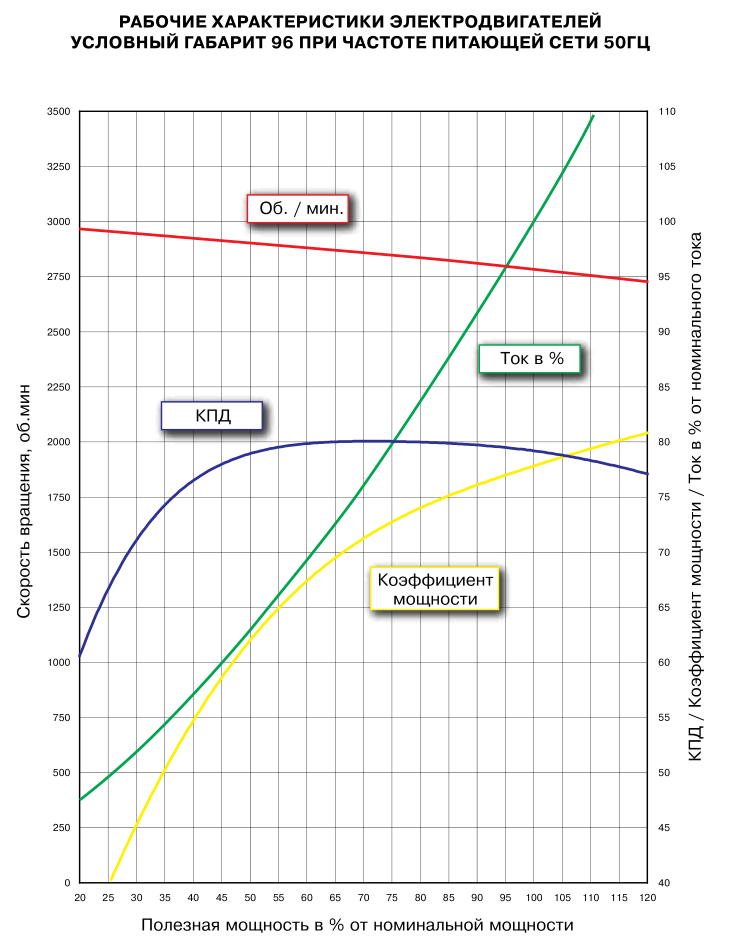
\includegraphics[width=0.6\linewidth]{novomet_motor_1}}
	\caption{Каталожные характеристики ПЭД}
	\label{ris:novomet_motor_1}
\end{figure}

Для асинхронных погружных двигателей производители в каталогах оборудования приводят характеристики позволяющие оценить КПД, потребляемый ток, частоту вращения вала и коэффициент электрической мощности от загрузки для определенной частоты вращения - рисунок \ref{ris:novomet_motor_1}. Нередко характеристики приводятся для двух частот вращения - 50Гц и 60 Гц.


Каталожная модель погружного АПЭД реализована в расчетных функциях \unf как модель двигателя с номером 1  \mintinline{vb.net}{motorID = 1}

Функции для расчета характеристик ПЭД начинаются с префикса \mintinline{vb.net}{motor_}. Описание функций можно найти в приложении "Автоматически сгенерированное описание".



\newpage
